
%%%%%%%%%%%%%%%%%%%%%%%%%%%%%%%%%%%%%%%%%%%%%%%%%%%%%%%%%%%%%%%%%%%%%%%%%%%%%%%%%%
\begin{frame}[fragile]\frametitle{}

\begin{center}
{\Large Text Pre-Processing with spaCy}

{\tiny (Ref: https://spacy.io/usage/spacy-101\#annotations)}

\end{center}


\end{frame}

%%%%%%%%%%%%%%%%%%%%%%%%%%%%%%%%%%%%%%%%%%%%%%%%%%%%%%%%%%%%%%%%%%%%%%%%%%%%%%%%%%
\begin{frame}[fragile]\frametitle{Text Pre-Processing}
Raw  text needs to be processed to bring it into ``normalized'' form. And some of the steps used are:

\begin{itemize}
\item Tokenization
\item Stemming
\item Lemmatization
\item \ldots
\end{itemize}
\end{frame}


%%%%%%%%%%%%%%%%%%%%%%%%%%%%%%%%%%%%%%%%%%%%%%%%%%%%%%%%%%%%%%%%%%%%%%%%%%%%%%%%%%
\begin{frame}[fragile]\frametitle{Tokenization}

\begin{lstlisting}
nlp = spacy.load('en_core_web_sm')
text = 'Apple is looking for buying a U.K. startup for $1 billion'
doc = nlp(text)
for token in doc:
    print(token.text)
		
Apple
is
looking
for
buying
a
U.K.
startup
for
$
1
billion

doc[0]
Apple

doc[2:5]
looking for buying
\end{lstlisting}
\end{frame}


%%%%%%%%%%%%%%%%%%%%%%%%%%%%%%%%%%%%%%%%%%%%%%%%%%%%%%%%%%%%%%%%%%%%%%%%%%%%%%%%%%
\begin{frame}[fragile]\frametitle{Tokenization}

\begin{itemize}
\item First, the raw text is split on whitespace characters, similar to \lstinline|text.split(' ')|.
\item Then checks each toekn if:
\begin{itemize}
\item Does the substring match a tokenizer exception rule? For example, “don’t” does not contain whitespace, but should be split into two tokens, “do” and “n’t”, while “U.K.” should always remain one token.
\item Can a prefix, suffix or infix be split off? For example punctuation like commas, periods, hyphens or quotes.
\end{itemize}

\item If there’s a match, the rule is applied and the tokenizer continues its loop, starting with the newly split substrings. 
\item This way, spaCy can split complex, nested tokens like combinations of abbreviations and multiple punctuation marks.
\item Each available language has its own subclass like English or German, that loads in lists of hard-coded data and exception rules.
\end{itemize}
\end{frame}

%%%%%%%%%%%%%%%%%%%%%%%%%%%%%%%%%%%%%%%%%%%%%%%%%%%%%%%%%%%%%%%%%%%%%%%%%%%%%%%%%%
\begin{frame}[fragile]\frametitle{Tokenization}

\begin{center}
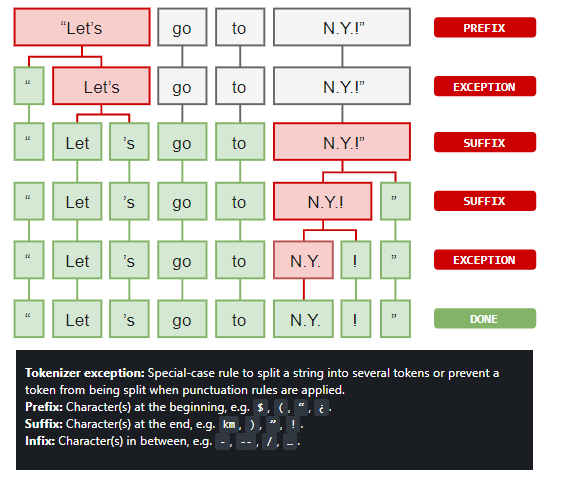
\includegraphics[width=0.7\linewidth,keepaspectratio]{spacy8}
\end{center}

\end{frame}


%%%%%%%%%%%%%%%%%%%%%%%%%%%%%%%%%%%%%%%%%%%%%%%%%%%%%%%%%%%%%%%%%%%%%%%%%%%%%%%%%%
\begin{frame}[fragile]\frametitle{Sentence Segmentation}

\begin{lstlisting}
text = 'Apple is looking for buying a U.K. startup. Government has given permission.'

doc = nlp(text)
for sent in doc.sents:
    print(sent)
		
Apple is looking for buying a U.K. startup.
Government has given permission.
\end{lstlisting}
	
\end{frame}


%%%%%%%%%%%%%%%%%%%%%%%%%%%%%%%%%%%%%%%%%%%%%%%%%%%%%%%%%%%%%%%%%%%%%%%%%%%%%%%%%%
\begin{frame}[fragile]\frametitle{ Stemming and Lemmatization}

Root word for ``Playing'' or ``Played'' is ``Play''. Thats the stem, a chopped version. Lemmatization is a bit advanced. It brings dictionary equivalent of the stem. spaCy has not given Stemming but only Lemmatization.


\begin{lstlisting}
doc1 = nlp("The striped bats are hanging on their feet for best")
for token in doc1:
  print(token.text, '\t', token.lemma_)
	
The 	 the
striped 	 stripe
bats 	 bat
are 	 be
hanging 	 hang
on 	 on
their 	 -PRON-
feet 	 foot
for 	 for
best 	 good
\end{lstlisting}


\end{frame}

%%%%%%%%%%%%%%%%%%%%%%%%%%%%%%%%%%%%%%%%%%%%%%%%%%%%%%%%%%%%%%%%%%%%%%%%%%%%%%%%%%
\begin{frame}[fragile]\frametitle{Stopwords}
Un-informative words to be skipped for text analysis.

\begin{lstlisting}
print(nlp.Defaults.stop_words)

print(len(nlp.Defaults.stop_words))
326 # in `sm' model

print(nlp.vocab['always'].is_stop())
True

nlp.Defaults.stop_words.add("asdf")
nlp.vocab['always'].is_stop = True # need to force it

nlp.Defaults.stop_words.remove("no")
nlp.vocab['no'].is_stop = False # need to force it

\end{lstlisting}

\end{frame}

%%%%%%%%%%%%%%%%%%%%%%%%%%%%%%%%%%%%%%%%%%%%%%%%%%%%%%%%%%%%%%%%%%%%%%%%%%%%%%%%%%
\begin{frame}[fragile]\frametitle{Matching }

  \begin{itemize}
    \item Rule-based (Token-based)
		\item Regex-based
		\item Phrase-based
  \end{itemize}
	

\end{frame}




%%%%%%%%%%%%%%%%%%%%%%%%%%%%%%%%%%%%%%%%%%%%%%%%%%%%%%%%%%%%%%%%%%%%%%%%%%%%%%%%%%
\begin{frame}[fragile]\frametitle{Token-based Matching }

  \begin{itemize}
    \item `Matcher' rules can refer to token annotations (e.g. the token text or tag\_, and flags (e.g. IS\_PUNCT).
		\item Lets you pass in a custom callback to act on matches – for example, to merge entities and apply custom labels
		\item To match large terminology lists, use the PhraseMatcher, which accepts Doc objects as match patterns
		\item Sample pattern \lstinline|[{"LOWER": "hello"}, {"IS_PUNCT": True}, {"LOWER": "world"}]|
  \begin{itemize}
    \item A token whose lowercase form matches “hello”, e.g. “Hello” or “HELLO”.
    \item A token whose is\_punct flag is set to True, i.e. any punctuation.
    \item A token whose lowercase form matches “world”, e.g. “World” or “WORLD”.
  \end{itemize}		
  \end{itemize}
	
\end{frame}


%%%%%%%%%%%%%%%%%%%%%%%%%%%%%%%%%%%%%%%%%%%%%%%%%%%%%%%%%%%%%%%%%%%%%%%%%%%%%%%%%%
\begin{frame}[fragile]\frametitle{Rule-based Matcher Explorer}

\begin{center}
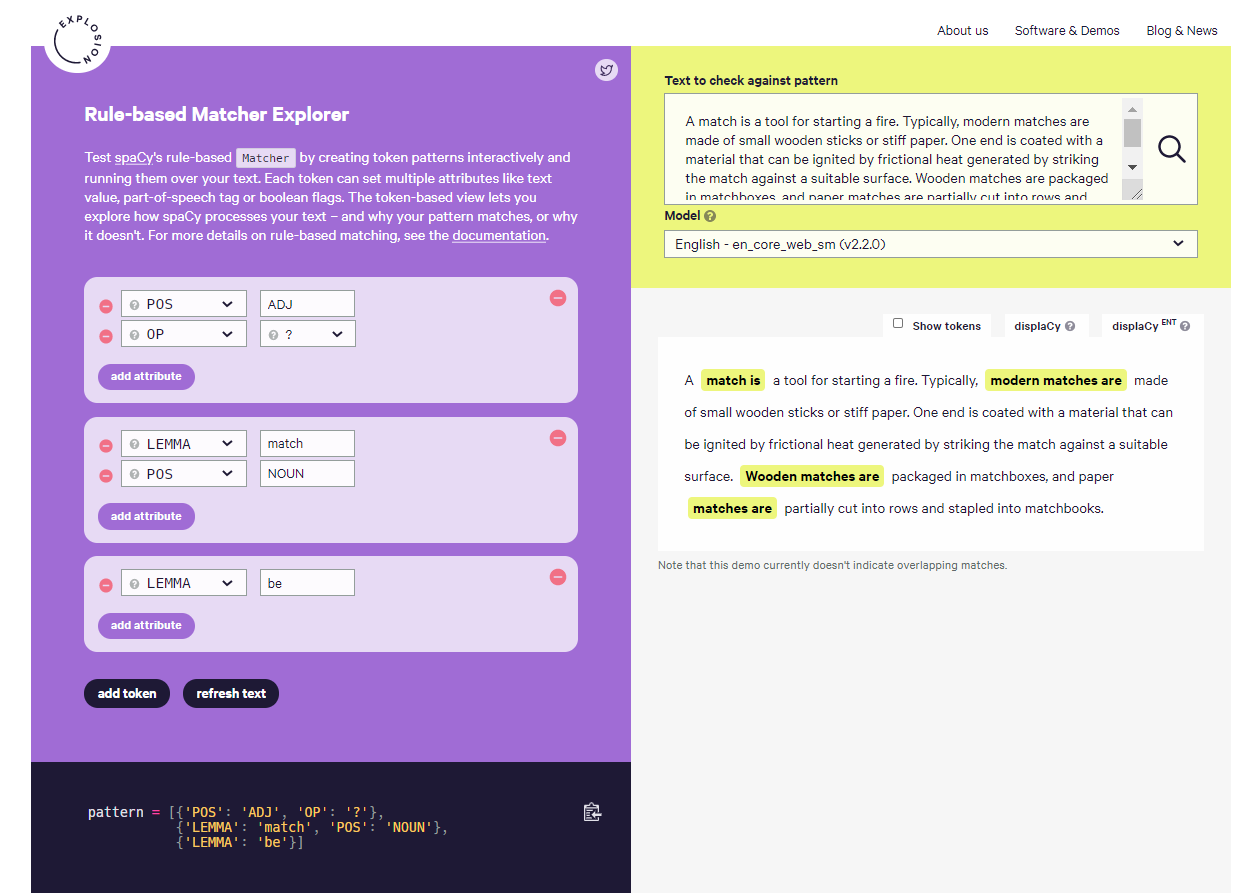
\includegraphics[width=0.8\linewidth,keepaspectratio]{spacy9}
\end{center}

{\tiny (Ref: https://explosion.ai/demos/matcher)}
\end{frame}


%%%%%%%%%%%%%%%%%%%%%%%%%%%%%%%%%%%%%%%%%%%%%%%%%%%%%%%%%%%%%%%%%%%%%%%%%%%%%%%%%%
\begin{frame}[fragile]\frametitle{Token-based matching }

\begin{lstlisting}
from spacy.matcher import Matcher
from spacy.tokens import Span
text = 'Hello, world! hello world'
doc = nlp(text)

pattern = [{'LOWER': 'hello'}, {'IS_PUNCT': True, 'OP': '?'}, {'LOWER': 'world'}]
matcher = Matcher(nlp.vocab)
matcher.add('hw', None, pattern)
matches = matcher(doc)
print(macthes)
[(17790654416186116455, 0, 3), (17790654416186116455, 4, 6)]

for match_id, start, end in matches:
    string_id = nlp.vocab.strings[match_id]
    span = doc[start:end]
    print(match_id, string_id, start, end, span.text)
		
17790654416186116455 hw 0 3 Hello, world
17790654416186116455 hw 4 6 hello world		
\end{lstlisting}
	
\end{frame}

%%%%%%%%%%%%%%%%%%%%%%%%%%%%%%%%%%%%%%%%%%%%%%%%%%%%%%%%%%%%%%%%%%%%%%%%%%%%%%%%%%
\begin{frame}[fragile]\frametitle{Regex-based matching }

In some cases, only matching tokens and token attributes isn’t enough, then comes REGEX operator which  operates on single tokens only. 

\begin{lstlisting}
pattern = [{"TEXT": {"REGEX": "^[Uu](\.?|nited)$"}},
           {"TEXT": {"REGEX": "^[Ss](\.?|tates)$"}},
           {"LOWER": "president"}]
\end{lstlisting}
	
	To match whole text use re.finditer
	
	\begin{lstlisting}
doc = nlp("The United States of America (USA) are commonly known as the United States (U.S. or US) or America.")

expression = r"[Uu](nited|\.?) ?[Ss](tates|\.?)"
for match in re.finditer(expression, doc.text):
    start, end = match.span()
    span = doc.char_span(start, end)
    # This is a Span object or None if match doesn't map to valid token sequence
    if span is not None:
        print("Found match:", span.text)
\end{lstlisting}

\end{frame}

%%%%%%%%%%%%%%%%%%%%%%%%%%%%%%%%%%%%%%%%%%%%%%%%%%%%%%%%%%%%%%%%%%%%%%%%%%%%%%%%%%
\begin{frame}[fragile]\frametitle{Example: Phone Numbers}



\begin{lstlisting}
matcher = Matcher(nlp.vocab)
pattern = [{"ORTH": "("}, {"SHAPE": "ddd"}, {"ORTH": ")"}, {"SHAPE": "ddd"},
           {"ORTH": "-", "OP": "?"}, {"SHAPE": "ddd"}]
matcher.add("PHONE_NUMBER", None, pattern)

doc = nlp("Call me at (123) 456 789 or (123) 456 789!")
print([t.text for t in doc])
matches = matcher(doc)
for match_id, start, end in matches:
    span = doc[start:end]
    print(span.text)
		
['Call', 'me', 'at', '(', '123', ')', '456', '789', 'or', '(', '123', ')', '456', '789', '!']
(123) 456 789
(123) 456 789		
\end{lstlisting}


\end{frame}



%%%%%%%%%%%%%%%%%%%%%%%%%%%%%%%%%%%%%%%%%%%%%%%%%%%%%%%%%%%%%%%%%%%%%%%%%%%%%%%%%%
\begin{frame}[fragile]\frametitle{Phrase Matching }

  \begin{itemize}
    \item To match large terminology lists, use the \lstinline|PhraseMatcher|
		\item Can give access to the tokens within the document and their relationships.
		\item Can easily access and analyze the surrounding tokens, merge spans into single tokens or add entries to the named entities in doc.ents.
  \end{itemize}
	
\end{frame}

%%%%%%%%%%%%%%%%%%%%%%%%%%%%%%%%%%%%%%%%%%%%%%%%%%%%%%%%%%%%%%%%%%%%%%%%%%%%%%%%%%
\begin{frame}[fragile]\frametitle{Phrase Matching }

\begin{lstlisting}
matcher = PhraseMatcher(nlp.vocab)
terms = ["Barack Obama", "Angela Merkel", "Washington, D.C."]
# Only run nlp.make_doc to speed things up
patterns = [nlp.make_doc(text) for text in terms]
matcher.add("TerminologyList", None, *patterns)

doc = nlp("German Chancellor Angela Merkel and US President Barack Obama "
          "converse in the Oval Office inside the White House in Washington, D.C.")
matches = matcher(doc)
for match_id, start, end in matches:
    span = doc[start:end]
    print(span.text)
		
Angela Merkel
Barack Obama
Washington, D.C.
\end{lstlisting}


\end{frame}


%%%%%%%%%%%%%%%%%%%%%%%%%%%%%%%%%%%%%%%%%%%%%%%%%%%%%%%%%%%%%%%%%%%%%%%%%%%%%%%%%%
\begin{frame}[fragile]
\frametitle{Next?}
 After the text preprocessing is done, the result may be used for more complicated NLP tasks, as features, such as for, machine classification, clustering etc, after doing vectorization.
\end{frame}